% multiple1902 <multiple1902@gmail.com>
% solution.tex
% Copyright 2011, multiple1902(Weisi Dai)
% https://bitbucket.org/multiple1902/beamerthemexjtu
%
% This work may be distributed and/or modified under the
% conditions of the LaTeX Project Public License, either version 1.3
% of this license or (at your option) any later version.
% The latest version of this license is in
%   http://www.latex-project.org/lppl.txt
% and version 1.3 or later is part of all distributions of LaTeX
% version 2005/12/01 or later.
%
% This work has the LPPL maintenance status `maintained'.
% 
% The Current Maintainer of this work is Weisi Dai.
%
\documentclass{beamer}

\graphicspath{{figures/}}
\hypersetup{pdfcreator=TeX,
%pdfpagemode = FullScreen,
}

\usepackage{amsthm}
\usepackage{fontspec,xltxtra,xunicode}
\usepackage[slantfont,boldfont]{xeCJK}
%\usepackage[slantfont]{xeCJK}
\usepackage{algorithm}
\usepackage{algorithmic}
\usepackage{tabularx}
\setmainfont{Times New Roman}%设置英文字体,不知道有什么用
\setCJKmainfont[BoldFont=SimSun]{SimSun} % 设置缺省中文字体

\usefonttheme[onlymath]{serif}%让字体变好看

%\newtheorem{theorem}{定理}[section]

%\newcommand{\suojin}{\hspace*{2em}}

\mode<presentation>
{
  \usetheme{XJTU}
  \useinnertheme{rounded}
  %\usefonttheme{serif}
}


\usepackage[english]{babel}
\usepackage[utf8]{inputenc}

\title[关于微分方程的辛方法和李群方法研究]
{关于微分方程的\\辛方法和李群方法研究}

%\subtitle{演講副標題} % (optional)

\author[卢燚]
{答辩人:卢燚} % {F.~Author\inst{1} \and S.~Another\inst{2}}

\institute[Xi'an Jiaotong University] % (optional, but mostly needed)
{
  %\inst{1}%
  %School of Electronic and Information Engineering\\
  %Xi'an Jiaotong University\\
  {\normalsize\textbf{指导教师:蒋耀林~教授}}
  %\and
  %\inst{2}%
  %Department of Theoretical Philosophy\\
  %University of Elsewhere
}

\date[Short Occasion] % (optional)
{西安交通大学数学与统计学院}

\subject{Subject} % meta info

\pgfdeclareimage[height=0.5cm]{university-logo}{inc/XJTU.eps}
\logo{\pgfuseimage{university-logo}}

\AtBeginSubsection[]
{
  \begin{frame}<beamer>{提纲}
    \tableofcontents[currentsection,currentsubsection]
  \end{frame}
}

%\beamerdefaultoverlayspecification{<+->}


\begin{document}

\begin{frame}
  \titlepage
\end{frame}

\begin{frame}{目录}
  \tableofcontents %[pausesections]
\end{frame}

\section{绪论}
\begin{frame}{1. 绪论}
\qquad 随着计算机软硬件的迅猛发展,计算机形态的日新月异,机器人科学和量子计算机的出现与
蓬勃发展,对高效高性能算法的研究变得越来越重要.性能好的便于求解的算法在工业生产中
起到了决定性的核心作用.算法的计算速度快,实现简单,性能稳定和可并行性已经成为许多领域里
的基本需求,拥有这些算法也就意味着拥有了国家的核心竞争力.

\qquad 本论文对与方程守恒性质相关的一些高性能算法(包括具有守恒性质或者近似有守恒性质微分方程的辛方法,
辛波形松弛方法),李群方法以及微分方程的李点对称方法展开研究,通过改进与创新,获得稳定的易于实现的数值
方法,和微分方程的一些守恒性质.所涉及的方向包括电路模拟,哈密尔顿系统的计算,流形上
的数值计算和偏微分方程的约化和解析解.
\end{frame}

\begin{frame}{1.1.1 电报方程背景及现状}
\qquad 电报方程,也称为传输线方程或电报员方程,来源于Maxwell方程组,是描述传输线中电流电压属性的一类方程.
更具体地讲,电报方程来源于这样的问题,导体由无限个二端口元件连接而成,每一个元件都是很小的传输线元件.

\begin{equation*}
\left\lbrace\begin{aligned}
	&\text{精确解}\\
	&\text{数值解}\left\lbrace\begin{aligned}
		&\text{解析方法:}\left\lbrace\begin{aligned}
			&\text{Exp-函数方法}\\
			&\text{Adomian 分解方法~(ADM)}\\
			&\text{变分迭代方法~(VIM)}\\
			&\text{同伦摄动方法~(HPM)}
		\end{aligned}
		\right.\\
		&\text{离散方法:}\left\lbrace \begin{aligned}
			&\text{微分二次方法~(DQM)}\\
			&\text{交替迭代隐式方法~(ADI)}\\
			&\text{WENO 方法}
		\end{aligned}
		 \right.
	\end{aligned}\right.
\end{aligned}  \right.
\end{equation*}

\end{frame}

\begin{frame}{1.1.2 拓展 QZK 方程背景及现状}
\qquad 拓展 quantum Zakharov-Kuznetsov~(QZK) 方程描述了等离子体里的物理现象.量子等离子体及其它们的性质获得了越来越多理论物理和实验物理领域的关注.

\qquad 本文所研究的 (2+1) 维拓展 QZK 方程的形式如下:
\begin{equation}\label{eq:eqzk}
u_{t}+auu_{x}+b(u_{xxx}+u_{yyy})+c(u_{xyy}+u_{xxy})=0,
\end{equation}
式中 $a,~b$ 和 $c$ 为常数, $u(x, y, t)$ 表示等离子体中电场波的势能.它是空间变量 $x,~y$ 和暂态变量 $t$ 的函数.方程 \eqref{eq:eqzk} 中的第一项为暂态发展项,系数 $a$ 和非线性项的系数 $b$ 和 $c$ 是多维空间扩散系数.

\qquad 针对上述方程,一些作者采用了极简形式的 Hirota 方法,得到了多孤子解和爆破解. 李点对称方法也有应用到方程 \eqref{eq:eqzk} 中的相关研究.
\end{frame}

\begin{frame}{1.1.3 哈密尔顿系统背景及现状}
\qquad 哈密尔顿系统是这样一类动力系统,该系统由哈密尔顿量 ${\displaystyle H({\boldsymbol {q}},{\boldsymbol {p}},t)}$ 所决定.该动力系统为状态变量 $\boldsymbol {q}$ 和 $\boldsymbol {p}$ 的方程,可写成
\begin{equation}\label{eq:hamiltonian}
\left\lbrace
\begin{aligned}
&{\frac {d{\boldsymbol {q}}}{dt}}=~~{\frac {\partial H}{\partial {\boldsymbol {p}}}},\\
&{\frac {d{\boldsymbol {p}}}{dt}}=-{\frac {\partial H}{\partial {\boldsymbol {q}}}}.
\end{aligned}
\right.
\end{equation}

\qquad 对于哈密尔顿系统,有一类比较成熟的,适于计算较长时间区间的方法,即辛方法.辛方法起源于冯康等人的工作, 其基本思想是避开盲目对精度的要求,巧妙地利用哈密尔顿系统的辛结构,将保持该结构作为目标,构造
数值格式.近些年的理论和数值算例都验证了该方法的优越性,系统的数值能量能够保持在系统的
真实值附近波动.
\end{frame}

\begin{frame}{1.2.1 辛方法}
\qquad 辛方法的定义是基于哈密尔顿系统的特性提出的.为了在数值计算上得到很好的效果,将辛格式定义为在
每个数值时间点上保持 $\boldsymbol {q}$ 与 $\boldsymbol {p}$ 的外微分二形式 $d\boldsymbol {q}_{n+1}\wedge d\boldsymbol {p}_{n+1}=d\boldsymbol {q}_n\wedge d\boldsymbol {p}_n$, 这里含有下指标的 $\boldsymbol {q}$ 和 $\boldsymbol {p}$
分别是在不同离散时间点上的广义位移和广义动量.

\qquad 为了容易验证辛格式,有一个与之等价的定义,即对于一个单步的数值方法 $z_{n+1}=\Phi_h(z_n)$, 其 Jacobian 矩阵是辛矩阵 
\begin{equation*}
(\nabla\Phi_h)^TJ^{-1}(\nabla\Phi_h)=J^{-1}.
\end{equation*}

\qquad 辛方法的数值格式有很多,包括隐式中点法,辛欧拉法, St\"{o}rmer-Verlet 方法,辛 Runge-Kutta 方法等.
\end{frame}

\begin{frame}{1.2.2 李群方法}
\qquad 李群方法联系着李群,李代数,指数映射,李点对称等,是指把李群作为变换群的一类方法的统称,包括流形上的李群方法和李点对称方法.

\qquad 李群是具有群结构的微分流形.作为群,李群有乘法和逆两个代数运算.作为
微分流形,李群的两个代数运算是光滑映射.

\qquad 李代数作为一个线性空间,其上包含一个双线性映射,称为李括号,满足反对称交换律和 Jacobi 恒等式.

\qquad 指数映射是连接李群和李代数的一个纽带,其定义为 $\mathrm{exp}: \mathfrak{g}\to \mathcal{G}$,
式中 $\mathfrak{g}=T\mathcal{G}$ 为 $\mathcal{G}$ 的切空间.这里我们要求有如下关系成立 $\mathrm{exp}(x)\mathrm{exp}(y)=\mathrm{exp}(xy)$. 矩阵李群是李群的一个特例,其群元素均为矩阵,对应的指数映射即为矩阵的指数函数
\begin{equation*}
	\mbox{expm}(A)=\sum_{j=0}^{\infty}\frac{A^j}{j!}.
\end{equation*}

\end{frame}

\begin{frame}{流形上的李群方法}
\qquad 本文中我们研究的李群方程是指在流形上的矩阵方程
\begin{equation*}
	Y'=A(t,Y)Y,\quad t\geq 0,\quad Y(0)=Y_0,
\end{equation*}
式中 $Y_0\in G $, $A:\mathbb{R}^+\times G\to \mathfrak{g}$, 这里的 $Y$ 和 $A(t,Y)$ 都是时间相关的 $N\times N$ 的矩阵.

\qquad 对于流形上的李群方程,我们知道其解的流随着时间依然保持在流形上.
然而,我们的数值计算都是在平直的欧氏空间上进行的,计算的结果也在全空间上,数值计算的
误差会导致计算结果并不在该流形上.

\qquad 为了解决这一类问题,有一类流形上的李群算法被
设计出来,这些算法能够很好地保证数值解落在流形上.由 Munthe-Kaas 提出的 Runge-Kutta Munthe-Kaas(RK-MK) 算法就是这样一类方法,利用了 Runge-Kutta 方法和指数映射的关系,使得数值解落在流形上.
\end{frame}

\begin{frame}{李点对称方法}
\qquad 李点对称方法基于单参数李群,将李群作用在微分方程上,能够达到求解微分方程特解
或者约化微分方程的效果.该方法体现了群在集合上的作用的思想.由于求导运算繁琐而有规律,该方法适合计算机程序进行计算.

\qquad 本文中,我们利用李点对称方法研究拓展 QZK 方程,研究了
偏微分方程的守恒性质,我们证明了 (2+1) 维拓展 QZK 方程是严格自共轭的,并且构造了其守恒律.
接着,我们给出了一维子代数最优系统.通过相应的相似变换, (2+1) 维拓展 QZK 方程
变为线性的偏微分方程.以上结果对研究该方程起到了积极的指导作用.
\end{frame}

\begin{frame}{1.2.3 波形松弛方法}
\qquad 波形松弛方法来源于对大规模集成电路系统的研究.该方法主要分为两个部分,对系统的分裂和对分裂后的系统迭代.首先,我们需要使用分裂函数
 将规模大的系统划分为较小规模的子系统,接下来是迭代,在系统之间交换信息,
直到收敛.由此可见,波形松弛方法的显著特性是问题解耦和潜在的可并行性.

\qquad 简而言之,波形松弛方法作为一个数学工具,通过函数的迭代来求解方程.首先选取分裂函数 $F(z,y)$ 使
得 $F(z,z)=f(z)$, 然后将方程中的 $f(z)$ 替换为 $F(z,y)$. 接下来为每一个子
系统选择一个合适的初始迭代,我们将 $F(z,y)$ 中的 $y$ 作为已知函数, $z$ 作为未知函数,进行迭代求解.
迭代的过程通常记作 $$\dot{z}^{k+1}=F(z^{k+1},z^{k}),$$ 式中 $k=0,1,\cdots$ 是迭代次数.
\end{frame}

\begin{frame}{1.3 本文的主要工作及创新}
\qquad 本文主要涉及了三部分内容,围绕辛方法和李群方法进行了研究,主要研究内容和创新点如下:

\begin{itemize}
\item (一) 我们提出了一种新的求解带有齐次边界条件的电报方程的方法.该方法有效地利用了一个变换,结合了辛方法的特性求解电报方程,得到了较好的数值效果.

\item (二) 我们将复合变分准则应用到了 (2+1) 维拓展 QZK 方程.应用这些李点对称,证明了该方程是自共轭的,并且构造了其守恒律.接着,给出了一维子代数最优系统,并通过相应的相似变换,将方程约化为线性的偏微分方程.

\item (三) 我们提出了求解哈密尔顿系统的辛波形松弛方法.该方法针对哈密尔顿系统给出了应该如何选择分裂函数的一种有效建议,求解过程中使用窗口加速技术.给出了系统哈密尔顿量在迭代下收敛到守恒的量的性质,并在数值结果中验证了这一点.
\end{itemize}
\end{frame}

\section{一类电报方程的辛方法研究}
\begin{frame}{一类电报方程的辛方法研究}
\begin{exampleblock}{}
\qquad Profound study of nature is the most fertile source of mathematical discoveries.\\
\flushright{--Joseph Fourier}
\end{exampleblock}
\end{frame}


\begin{frame}{2 一类电报方程的辛方法研究}
\qquad 本章所研究的是这样一类电报方程
\begin{equation}\label{eq:tele}
\left\lbrace
\begin{aligned}
&\frac{\partial ^2 w(x,t)}{\partial t^2}+k\frac{\partial w(x,t)}{\partial t}=a^2 \frac{\partial ^2 w(x,t)}{\partial x^2} + b w(x,t),\\
&\begin{aligned}
w(x,0)&=g_1(x),&0 \le x \le 1,\\
w_t(x,0)&=g_2(x),&0 \le x \le 1,\\
w(0,t)&=0,&0 \le t \le T,\\
w(1,t)&=0,&0 \le t \le T,
\end{aligned}
\end{aligned}
\right.
\end{equation}
式中 $k > 0$, $a>0$ 和 $b < 0$ 是常数. $g_1(x)$ 和 $g_2(x)$ 是光滑函数, 满足相容性条件 $g_1(0)=0$. $w(x,t) \in \mathbb{R}$ 为所求函数.
\end{frame}

\begin{frame}{2.1 辛的基本概念}
\begin{definition}[辛方法]
一个单步的数值方法 $z_{n+1}=\Phi_h(z_n)$ 称为辛方法,如果该方法保持二形式
\begin{equation*}
dq_{n+1}\wedge dp_{n+1}=dq_n\wedge dp_n,
\end{equation*}
式中 $z_n=(q_n;p_n),~n=1,2,\cdots$.
\end{definition}

下面是辛方法的一个等价定义.

\begin{definition}[辛方法]\label{def:symplectic}
一个单步的数值方法 $z_{n+1}=\Phi_h(z_n)$ 称之为辛方法,如果 $\Phi_h$ 的 Jacobian 矩阵满足
\begin{equation*}
(\nabla\Phi_h)^TJ^{-1}(\nabla\Phi_h)=J^{-1}.
\end{equation*}
\end{definition}
\end{frame}

\begin{frame}{2.1 辛的基本概念}
\qquad 在这里给出一些辛方法的例子.

\begin{itemize}
\item 隐式中点法
\begin{equation*}
\frac{z^{n+1}-z^n}{\tau}=J^{-1}H_z(\frac{z^{n+1}+z^n}{2}),
\end{equation*}
为二阶辛方法.

\item 辛欧拉法
\begin{equation*}
\begin{aligned}
p_{n+1}&=p_n-hH_q(p_{n+1},q_n),\\
q_{n+1}&=q_n+hH_p(p_{n+1},q_n),
\end{aligned}
\quad \text{or} \quad
\begin{aligned}
p_{n+1}&=p_n-hH_q(p_n,q_{n+1}),\\
q_{n+1}&=q_n+hH_p(p_n,q_{n+1}),
\end{aligned}
\end{equation*}
均为一阶方法.
\end{itemize}

\end{frame}

\begin{frame}{2.1 辛的基本概念}
\begin{itemize}
\item 辛 Runge-Kutta 方法

\qquad 对于 Runge-Kutta 方法,可以知道, $\nu$ 步的 Runge-Kutta 方法可以写成
\begin{equation*}
  \left\lbrace
    \begin{aligned}
      Y_{n+1}^{r}&=\eta(t_{n})+h\sum_{s=1}^{\nu}a_{rs}f(t_{n+1}^{s},Y_{n+1}^{s}),\quad r=1,\cdots, \nu, \\
      \eta(t_{n+1})&=\eta(t_{n})+h\sum_{s=1}^{\nu}b_{s}f(t_{n+1}^{s},Y_{n+1}^{s}).
    \end{aligned}
  \right.
\end{equation*}

\qquad 其对应的 Butcher 表可以写成

\begin{center}
  \begin{tabular}{c|cccc}
    $c_1$&$a_{11}$&$a_{12}$&$\cdots$&$a_{1\nu}$\\
    $c_2$&$a_{21}$&$a_{22}$&$\cdots$&$a_{2\nu}$\\
    $\vdots$&$\vdots$&$\vdots$&$\ddots$&$\vdots$\\
    $c_{\nu}$&$a_{\nu 1}$&$a_{\nu 2}$&$\cdots$&$a_{\nu \nu}$\\
    \hline
         &$b_{1}$&$b_{2}$&$\cdots$&$b_{\nu}$
  \end{tabular}
\end{center}
\end{itemize}
\end{frame}

\begin{frame}{2.2 电报方程的辛方法}
\qquad 算法基本分三个步骤,即做变换,离散求解哈密尔顿系统,做逆变换得到数值解.

%\begin{algorithm}
%\caption{电报方程求解基本算法}
\begin{block}{电报方程求解基本算法}
\begin{algorithmic}[1]
\STATE 将电报方程 \eqref{eq:tele} 变换成相应的 Klein-Gordon 方程. 相应地改变初边值条件. \newline
\STATE 离散得到的 Klein-Gordon 方程写成哈密尔顿方程组. 使用辛方法求解该哈密尔顿系统,得到 Klein-Gordon 方程的数值解. \newline
\STATE 对该数值解作用逆变换,得到电报方程的数值解.
\end{algorithmic}
\end{block}
%\label{alg:tele}
%\end{algorithm}

\end{frame}

\begin{frame}{2.2 电报方程的辛方法}
现在回忆一下电报方程 \eqref{eq:tele}, 针对电报方程 \eqref{eq:tele} 本身来看,
\begin{equation}\label{eq:telegraph}
\frac{\partial ^2 w}{\partial t^2}+k\frac{\partial w}{\partial t}=a^2 \frac{\partial ^2 w}{\partial x^2} + b w.
\end{equation}

\begin{lemma}[由电报方程到 Klein-Gordon 方程的变换]\label{thm:trans}
\emph{令 $w=e^{-\frac{1}{2}kt}u$, 电报方程 \eqref{eq:telegraph} 将变换成为如下的 Klein-Gordon 方程
\begin{equation}\label{eq:kg}
\frac{\partial ^2 u}{\partial t^2}=a^2 \frac{\partial ^2 u}{\partial x^2} + (b+\frac{1}{4}k^2) u.
\end{equation}}
\end{lemma}
其逆变换可以由该变换直接得出,对于 $n$ 维情形,也可以得到相应的变换.
\end{frame}

\begin{frame}{2.2 电报方程的辛方法}
\qquad 离散的过程,取 $0=x_0<x_1<\cdots<x_{N-1}<x_N=1,$ 式中 $x_i=i\Delta x,~i = 1,2,\cdots,N$.

\qquad 令 $u_i(t)=u(x_i,t)$, $U=(u_1,u_2,\cdots,u_{N-1})^T$, 离散的结果对应着如下的二阶 ODE
\begin{equation}\label{eq:aftert}
\left\lbrace
\begin{aligned}
&\frac{d^2U}{dt^2}=(-a^2 S+(b+\frac{1}{4}k^2)I) U,\\
&\begin{aligned}
U(0)=&(g_1(x_1),g_1(x_2),\cdots,g_1(x_{N-1}))^T,\\
U_t(0)=&(g_2(x_1)+\frac{1}{2}kg_1(x_1),g_2(x_2)\\
    &+\frac{1}{2}kg_1(x_2),\cdots,g_2(x_{N-1})+\frac{1}{2}kg_1(x_{N-1}))^T.
\end{aligned}
\end{aligned}
\right.
\end{equation}
\end{frame}

\begin{frame}{2.2 电报方程的辛方法}
令 $q(t)=U(t),~ p(t)=U_t(t)$, 可以把二阶 ODE 写成如下形式
\begin{equation}\label{eq:ode}
\left\lbrace
\begin{aligned}
\frac{dq}{dt}&=p,\\
\frac{dp}{dt}&=-Mq,
\end{aligned}
\right.
\end{equation}
式中 $M=a^2 S-(b+\frac{1}{4}k^2)I.$
系统的哈密尔顿量为
\begin{equation*}
H=\frac{1}{2}p^Tp+\frac{1}{2}q^TMq.
\end{equation*}
\end{frame}

\begin{frame}{2.2 电报方程的辛方法}
\qquad 在数学上, Courant-Friedrichs-Lewy~(CFL) 条件是保证数值格式收敛的必要条件.通常,时间步长必须取得足够小,才能保证计算过程中结果收敛.

\qquad 因为 Klein-Gordon 方程和波动方程有相似的类型,取波动方程的 CFL 条件作为 Klein-Gordon 方程的 CFL 条件
\begin{equation*}
a^2\frac{\Delta t^2}{\Delta x^2}\le 1.
\end{equation*}

\begin{theorem}[算法的阶]\label{thm:tele}
\emph{算法在空间上是 $2$ 阶的,时间上是 $k$ 阶的,这里 $k$ 为辛格式的阶数.}
\end{theorem}
\end{frame}

\begin{frame}{2.3 数值实验1}
在此例子中,取方程 \eqref{eq:telegraph} 中的参数为 $k = 8\pi,~a = 2$ 和 $b
= -3\pi^2$. 此例的精确解是 $w(x,t) = e^{-\pi t}sin(\pi x)$. 初值和边值条件分别为
\begin{equation*}
\begin{aligned}
w(x,0)&=\sin(\pi x),\\
w_t(x,0)&=-\pi \sin(\pi x),
\end{aligned}
\end{equation*}
和
\begin{equation*}
\begin{aligned}
w(0,t)&=0,\\
w(1,t)&=0.
\end{aligned}
\end{equation*}

通过变换 $w = e^{-4\pi t}u$, 得到方程 \eqref{eq:kg}, 其中初值条件为
\begin{equation*}
\begin{aligned}
u(x,0)&=\sin(\pi x),\\
u_t(x,0)&=3\pi \sin(\pi x),
\end{aligned}
\end{equation*}
边值条件为
\begin{equation*}
\begin{aligned}
u(0,t)&=0,\\
u_t(1,t)&=0.
\end{aligned}
\end{equation*}
\end{frame}

\begin{frame}{2.3 数值实验1}
\textbf{$\Delta x$ 的阶}
\begin{table}[h]
  \centering
\caption{误差无穷范数随 $\Delta x$ 的变化情况,其中 $\Delta t=0.001$, $T=2$}
\begin{tabularx}{\linewidth}{XXXXX}
 \hline
 $\Delta x$ &直接方法 & 辛欧拉 & 隐式中点 & St\"{o}rmer-Verlet\\
 \hline
 0.1 & 0.0026 & 0.0011 & 0.0025 & 0.0017\\
 0.05 & 0.0010 & 0.0013 & 0.0012 & 4.2103e-04\\
 0.025 & 6.8722e-04 & 0.0014 & 9.2472e-04 & 1.0098e-04\\
 0.0125 & 6.0390e-04 & 0.0015 & 8.4536e-04 & 2.1029e-05\\
 0.00625 & 5.8372e-04 & 0.0015 & 8.2554e-04 & 3.5435e-06\\
 \hline
\end{tabularx}
  \label{tab:dx1}
\end{table}
\end{frame}

\begin{frame}{2.3 数值实验1}
\textbf{$\Delta t$ 的阶}

\begin{table}[h]
  \centering
\caption{误差的无穷范数随 $\Delta t$ 的变化情况,其中 $\Delta x=0.01$, $T=2$}
\begin{tabularx}{\linewidth}{XXXXX}
 \hline
 $\Delta t$ &直接方法 & 辛欧拉 & 隐式中点 & St\"{o}rmer-Verlet\\
 \hline
 0.01 & 0.0057 & - & 8.3585e-04 & - \\
 0.005 & 0.0029 & 0.0074 & 2.2122e-04 & 1.5288e-04 \\
 0.0025 & 0.0015 & 0.0037 & 6.7965e-05 & 3.0713e-05 \\
 0.00125 & 7.3818e-04 & 0.0018 & 2.9746e-05 & 8.5729e-06 \\
 0.000625 & 3.7797e-04 & 9.0788e-04 & 2.0234e-05 & 1.4851e-05 \\
 \hline
\end{tabularx}
  \label{tab:dt1}
\end{table}
\end{frame}

\begin{frame}{2.3 数值实验1}
\textbf{长时间性质}

\begin{table}[h]
  \centering
\caption{误差的无穷范数随 $T$ 的变化情况,其中 $\Delta x=0.05$, $\Delta t=0.001$}
\begin{tabularx}{\linewidth}{XXXXX}
 \hline
 $T$ &直接方法 & 辛欧拉 & 隐式中点 & St\"{o}rmer-Verlet\\
 \hline
 1 & 0.0010 & 0.0013 & 4.3489e-04 & 1.7282e-04 \\
 10 & 0.0010 & 0.0013 & 4.3489e-04 & 4.2674e-04 \\
 100 & 0.0010 & 0.0013 & 4.3489e-04 & 4.2674e-04 \\
 1000 & 0.0010 & 0.0013 & 4.3489e-04 & 4.2674e-04 \\
 10000 & 0.0010 & 0.0013 & 4.3489e-04 & 4.2674e-04 \\
 \hline
\end{tabularx}
  \label{tab:t1}
\end{table}
\end{frame}

\begin{frame}{2.3 数值实验2}
在此例子中,我们求解二维的电报方程,
\begin{equation*}
\frac{\partial ^2 w}{\partial t^2}+8\pi \frac{\partial w}{\partial
t}=4 (\frac{\partial ^2 w}{\partial x^2} + \frac{\partial ^2
w}{\partial y^2}) -3\pi^2 w.
\end{equation*}
精确解为 $w(x,t) = e^{-\pi t}sin(\pi x)sin(\pi y)$.
\end{frame}

\begin{frame}{2.3 数值实验2}
\textbf{$\Delta x$ 的阶}

\begin{table}[h!]
  \centering
\caption{误差的无穷范数随 $\Delta x$ 的变化情况.其中 $\Delta t=0.001$, $T=2$}
\begin{tabularx}{\linewidth}{XXXXX}
 \hline
 $\Delta x$ &直接方法 & 辛欧拉 & 隐式中点 & St\"{o}rmer-Verlet\\
 \hline
 0.1 & 0.8252 & 0.0018 & 0.0017 & 0.0017\\
 0.05 & 0.8301 & 5.0684e-04 & 4.2688e-04 & 4.2674e-04\\
 0.025 & 0.8314 & 2.0812e-04 & 1.0680e-04 & 1.0667e-04\\
 0.0125 & 0.8317 & 1.5813e-04 & 2.6763e-05 & 2.6625e-05\\
 \hline
\end{tabularx}
  \label{tab:dx3}
\end{table}
\end{frame}

\begin{frame}{2.3 数值实2}
\textbf{$\Delta t$ 的阶}

\begin{table}[h]
  \centering
\caption{误差的无穷范数随 $\Delta t$ 的变化情况.其中 $\Delta x=0.01$, $T=1$}
\begin{tabularx}{\linewidth}{XXXXX}
 \hline
 $\Delta t$ &直接方法 & 辛欧拉 & 隐式中点 & St\"{o}rmer-Verlet\\
 \hline
 0.001 & 0.8317 & 0.0015 & 2.5175e-05 & 1.1497e-05 \\
 0.0005 & 0.8317 & 7.3588e-04 & 1.9097e-05 & 1.5646e-05 \\
 0.00025 & 0.8317 & 3.7202e-04 & 1.7581e-05 & 3.0713e-05 \\
 0.000125 & 0.8317 & 1.8992e-04 & 1.7203e-05 & 8.5729e-06 \\
 \hline
\end{tabularx}
  \label{tab:dt3}
\end{table}
\end{frame}

\begin{frame}{2.3 数值实验2}
\textbf{长时间性质}

\begin{table}[h]
  \centering
\caption{误差的无穷范数随 $T$ 的变化情况.其中 $\Delta x=0.1$, $\Delta t=0.001$}
\begin{tabularx}{\linewidth}{XXXXX}
 \hline
 $T$ &直接方法 & 辛欧拉 & 隐式中点 & St\"{o}rmer-Verlet\\
 \hline
 1 & 0.8252 & 0.0026 & 0.0017 & 0.0017 \\
 10 & 0.8599 & 0.0026 & 0.0017 & 0.0017 \\
 100 & 0.8599 & 0.0026 & 0.0017 & 0.0017 \\
 1000 & 0.8599 & 0.0026 & 0.0017 & 0.0017 \\
 \hline
\end{tabularx}
  \label{tab:t3}
\end{table}
\end{frame}

\section{基于李群方法的拓展 QZK 方程研究}
\begin{frame}{基于李群方法的拓展 QZK 方程研究}
\begin{exampleblock}{}
\qquad Among all of the mathematical disciplines the theory of differential equations is the most important... It furnishes the explanation of all those elementary manifestations of nature which involve time.
\flushright{--Sophus Lie}
\end{exampleblock}
\end{frame}

\begin{frame}{3 基于李群方法的拓展 QZK 方程研究}
\qquad 本章对如下形式的 (2+1) 维拓展 QZK 方程进行讨论,得到了一些该方程的可参考的结论
\begin{equation*}
u_{t}+auu_{x}+b(u_{xxx}+u_{yyy})+c(u_{xyy}+u_{xxy})=0.
\end{equation*}
\end{frame}

\begin{frame}{3.1 李点对称方法}
\qquad 无穷小变换是李群方法的基础,可以说,无穷小变换包含了李群方法几乎所有需要的量.

\qquad 对单参数李变换群
\begin{equation}\label{eq:liet}
x^{*}=X(x;\varepsilon)
\end{equation}
中的 $\varepsilon$ 在 $\varepsilon=0$ 处展开,取到一阶项
\begin{equation*}
x+\varepsilon \xi(x),
\end{equation*}
式中
\begin{equation*}
\xi(x)=\left.\frac{\partial X(x;\varepsilon)}{\partial \varepsilon}\right|_{\varepsilon=0}.
\end{equation*}
称 $x+\varepsilon \xi(x)$ 为单参数李变换群的\textbf{无穷小变换}.

\qquad 可以看到,无穷小变换包含了单参数李变换群的直到一阶导数性质,这对应着研究李群上的切空间,即李代数.
\end{frame}

\begin{frame}{3.1 李点对称方法}
\qquad 李点对称方法基于三个李基本定理,为了引入微分方程的不变性,首先引入不变函数的概念.
\begin{definition}[不变函数]
	一个无穷可微函数 $F(\mathbf{x})$ 叫做李群作用下的不变函数,当且仅当对于任意群变换,有
	\begin{equation*}
		F(\mathbf{x^*})\equiv F(\mathbf{x}).
	\end{equation*}
如果 $F(\mathbf{x})$ 是群作用下的不变函数,称 $F(\mathbf{x})$ 是群作用下的不变量,也称 $F(\mathbf{x})$ 在群作用下是不变的.
\end{definition}

定义 $\boldsymbol {X}=\Sigma \xi_i(x)\frac{\partial}{\partial x_i}$, 对于不变函数,有如下定理.
\begin{theorem}
\emph{	$F(\mathbf{x})$ 在群的作用下是不变的,当且仅当
	\begin{equation*}
		\boldsymbol {X}F(\mathbf{x})\equiv 0.
	\end{equation*}}%
\end{theorem}
\end{frame}

\begin{frame}{3.1 李点对称方法}
对于偏微分方程,给出不变解的概念.
\begin{definition}[不变解]
	$u=\Theta(x)$ 是被单参数李群所接受的偏微分方程的不变解,当且仅当
	\begin{description}
		\item[(1)] $u=\Theta(x)$ 是无穷小变换的不变解.
		\item[(2)] $u=\Theta(x)$ 是偏微分方程的解.
	\end{description}
\end{definition}

根据定义,可以看到, $u=\Theta(x)$ 是不变解,当且仅当
\begin{description}
	\item[(1)] 当 $u=\Theta(x)$ 时 $X(u-\Theta(x))=0$, 即
	\begin{equation*}
		\xi_i(x,\Theta(x))\frac{\partial \Theta(x)}{\partial x_i}=\eta(x,\Theta(x)).
	\end{equation*}
	\item[(2)] 当 $u=\Theta(x)$ 时, $F(x,u,\partial u,\cdots,\partial ^k u)=0$ 即
	\begin{equation*}
		F(x,\Theta(x),\partial \Theta(x),\cdots,\partial ^k \Theta(x))=0.
	\end{equation*}
\end{description}
\end{frame}

\begin{frame}{3.2 拓展 QZK 方程的李群方法主要结果}
\qquad 定义 $m$ 个含有 $n$ 个独立自变量的 $r$ 阶  ($r\geq1$) PDE 系统为
\begin{equation}\label{eq:system}
F_\alpha(x,u,u_{(1)},\cdots,u_{(r)})=0,~ \alpha=1,2,\cdots,m,
\end{equation}
式中, $x$ 为自变量,其分量为 $x^i$, $u$ 为因变量,其分量为 $u^\beta$.

\begin{definition}[形式 Lagrangian]
	方程 \eqref{eq:system} 的形式 Lagrangian 定义为
	\begin{equation*}
		L=vF(x,u,u_{(1)},\cdots,u_{(r)}),
	\end{equation*}
	式中 $v$ 是一个新的因变量.
\end{definition}

\qquad 向量 $C=(C^1,C^2,\cdots,C^n)$ 是系统 \eqref{eq:system} 的守恒向量,如果在系统 \eqref{eq:system} 的解空间上满足
\begin{equation}\label{eq:div}
divC\equiv D_i(C^i)=0.
\end{equation}
我们说表达式 \eqref{eq:div} 是系统 \eqref{eq:system} 的一个守恒律.
\end{frame}

\begin{frame}{3.2 拓展 QZK 方程的李群方法主要结果}
\qquad 可以根据如下定理获得守恒量

\begin{theorem}
\emph{系统 \eqref{eq:system} 的李点对称算子能够由下面的公式得到一个守恒向量 $C=(C^1,C^2,\cdots,C^n)$
\begin{equation*}
\begin{aligned}
C^i&=L\xi^i+W^\alpha \bigg[\frac{\partial L}{\partial u^\alpha_i}-D_j(\frac{\partial L}{\partial u^\alpha_{ij}})+D_jD_k(\frac{\partial L}{\partial u^\alpha_{ijk}})-\cdots\bigg]\\
&+D_j(W^\alpha)\bigg[\frac{\partial L}{\partial u^\alpha_{ij}}-D_k(\frac{\partial L}{\partial u^\alpha_{ijk}})+\cdots\bigg]+D_jD_k(W^\alpha)\bigg[\frac{\partial L}{\partial u^\alpha_{ijk}}\bigg]+\cdots,\\
\end{aligned}
\end{equation*}
式中 $W^\alpha=\eta^\alpha-\xi^ju^\alpha_j$ 和 $L=v^\alpha F_\alpha(x,u,v,u_{(1)},v_{(1)},\cdots,u_{(r)},v_{(r)})$, 是系统的形式 Lagrangian.其中 $v= (v^1,v^2,\cdots,v^m)$ 是对偶变量, $\alpha=1,2,\cdots, m$.}
\end{theorem}
\end{frame}

\begin{frame}{3.2 拓展 QZK 方程的李群方法主要结果}
\qquad 首先给出严格自共轭的定义,然后要证明方程 \eqref{eq:eqzk} 是严格自共轭的.

\begin{definition}[严格自共轭]
	微分方程 \eqref{eq:system} 是严格自共轭的,如果令 $v=u$, 其所有的解 $u$ 均满足自共轭方程.
\end{definition}

\qquad 根据此定义,可以验证

\begin{theorem}
\emph{方程 \eqref{eq:eqzk} 是严格自共轭的.}
\end{theorem}
\end{frame}

\begin{frame}{3.2 拓展 QZK 方程的李群方法主要结果}
\qquad 接下来,根据 Ibragimov 的思想,构造方程 \eqref{eq:eqzk} 新的守恒律.根据李点对称方法,方程 \eqref{eq:eqzk} 的李点对称表示为
\begin{align*}
	X_{1}&=\frac{\partial}{\partial x},~X_{2}=\frac{\partial}{\partial y},~X_{3}=\frac{\partial}{\partial t},\\
	X_{4}&=x\frac{\partial}{\partial x}+3t\frac{\partial}{\partial t}+y\frac{\partial}{\partial y}-2u\frac{\partial}{\partial u},\\
	X_{5}&=t\frac{\partial}{\partial x}+\frac{1}{a}\frac{\partial}{\partial u}.
\end{align*}
\end{frame}

\begin{frame}{3.2 拓展 QZK 方程的李群方法主要结果}
\begin{itemize}
 \item[(1)] 首先考虑方程 \eqref{eq:eqzk} 的李点对称 $X_{1}=\frac{\partial}{\partial x}$. 其守恒向量的分量为
\begin{equation*}
\begin{aligned}
c^{x}&=uu_t-cu_xu_{yy}+cu_yu{xx}+cu_yu_{xy};\\
c^{y}&=-bu_xu{yy}+cu{xx}u_y+bu_yu_{xy}-cu_yu_{xxx}-cu_yu_{xxy}-buu_{xyy};\\
c^{t}&=-uu_x.
\end{aligned}
\end{equation*}
 \item[(2)] 类似地, $X_{2}=\frac{\partial}{\partial y}$ 对应的李点对称守恒向量为
\begin{equation*}
\begin{aligned}
c^{x}&=-a^2u_y-bu_yu_{xx}+bu_xu_{xy}+cu_xu_{yy}-buu_{xxy}-cuu_{xyy}-cuu_{yyy};\\
c^{y}&=uu_t+au^2u_x+bu_{xxx}-cu_yu_{xx}+cu_xu_{xy}+cu_xu_{yy};\\
c^{t}&=-uu_y.
\end{aligned}
\end{equation*}
\end{itemize}
\end{frame}

\begin{frame}{3.2 拓展 QZK 方程的李群方法主要结果}
\begin{itemize}
\item[(3)] 对应于 $X_{3}=\frac{\partial}{\partial t}$, 有如下结果
\begin{equation*}
\begin{aligned}
c^{x}&=-au^2u_t-bu_{xx}u_t-cu_{xy}u_t-cu_{yy}u_t+bu_{xt}u_x+cu_{tx}u_y+cu_{ty}u_x\\
&~~~~+cu_{ty}u_y-buu_{xxt}-cuu_{txy}-cuu_{tyy};\\
c^{y}&=-cu_tu_{xx}-cu_{xt}u_t-bu_{yy}u_t+cu_xu_{tx}+cu_yu_{tx}+cu_xu_{ty}+bu_yu_{ty}\\
&~~~~-cuu_{txx}-cuu_{txy}-buu_{tyy};\\
c^{t}&=au^2u_x+buu_{xxx}+buu_{yyy}+cuu_{xyy}+cuu_{xxy}.
\end{aligned}
\end{equation*}
\end{itemize}
\end{frame}

\begin{frame}{3.2 拓展 QZK 方程的李群方法主要结果}
\begin{itemize}
\item[(4)] 对应于 $X_{4}=x\frac{\partial}{\partial x}+3t\frac{\partial}{\partial t}+y\frac{\partial}{\partial y}-2u\frac{\partial}{\partial u}$, 守恒向量为
\begin{equation*}
\begin{aligned}
c^{x}&=xu(u_{t}+auu_{x}+bu_{yyy})-(2u+xu_{x}+yu_{y}+3tu_{t})(au^2+bu_{xx}\\
&+cu_{xy}+cu_{yy})+(3u_{x}+xu_{xx}+yu_{xy}+3tu_{tx})(bu_{x}+cu_{y})\\
&+(3u_{y}+xu_{xy}+yu_{yy}+3tu_{ty})(cu_{x}+cu_{y})-(4u_{xx}+yu{xxy}\\
&+3tu_{txx})bu-(4u_{xy}+yu{xyy}+3tu_{txy})cu\\
&-(4u_{yy}+yu{yyy}+3tu_{tyy})cu;\\
c^{y}&=yu(u_{t}+auu_{x}+bu_{xxx})-(2u+xu_{x}+yu_{y}+3tu_{t})(cu_{xx}+cu_{xy}\\
&+bu_{yy})+(3u_{x}+xu_{xx}+yu_{xy}+3tu_{tx})(cu_{x}+cu_{y})+(3u_{y}+xu_{xy}\\
&+yu_{yy}+3tu_{ty})(cu_{x}+bu_{y})-(4u_{xx}+xu_{xxx}+3tu_{txx})cu\\
&-(4u_{xy}+xu_{xxy}+3tu_{txy})cu-(4u_{yy}+xu_{xyy}+3tu_{tyy})bu;\\
c^{t}&=3btuu_{t}u_{xxx}+3(b+c)tuu_{yyy}+3ctuu_{xyy}-3atu^2uu_x\\
&-2xuu_x-yu_y-2u^2.
\end{aligned}
\end{equation*}
\end{itemize}
\end{frame}

\begin{frame}{3.2 拓展 QZK 方程的李群方法主要结果}
\begin{itemize}
\item[(5)] 最后,考虑 $X_{5}=t\frac{\partial}{\partial x}+\frac{1}{a}\frac{\partial}{\partial u}$, 可以得到
\begin{equation*}
\begin{aligned}
c^{x}&=btuu_{yyy}+ctuu_{xyy}-ctu_{x}u_{xx}-ctu_{x}u_{yy}+ctu_{y}u_{xx}+\frac{b}{a}u_{xx}+\frac{c}{a}u_{xy}\\
&~~~~+\frac{c}{a}u_{yy}+tuu_t+u^2;\\
c^{y}&=\frac{c}{a}u_{xx}+\frac{c}{a}u_{xy}+\frac{b}{a}u_{yy}-ctu_{x}u_{xy}-btu_{x}u_{yy}+ctu_{y}u_{xx}\\
&~~~~-ctuu_{xxx}-ctuu_{xxy};\\
c^{t}&=\frac{1}{a}u-tu_{x}u.\\
\end{aligned}
\end{equation*}
\end{itemize}
\end{frame}

\begin{frame}{3.2 拓展 QZK 方程的李群方法主要结果}
\qquad 接下来,来构造方程 \eqref{eq:eqzk} 的一维子代数最优系统.有如下结果
\begin{theorem}
\emph{方程 \eqref{eq:eqzk} 的一个一维子代数最优系统为
\begin{equation*}
	mX_{3}+nX_{4}+X_{5},~ X_{4}, X_{3},~ X_{3}-X_{2}, ~X_{3}+X_{2}, ~lX_{1}+X_{2}, ~X_{1},
\end{equation*}
式中 $m,n,l\in \mathbf{R}$ 为任意非零常数.}
\end{theorem}
\end{frame}

\begin{frame}{3.2 拓展 QZK 方程的李群方法主要结果}
\qquad 根据得到的一维子代数来约化方程 \eqref{eq:eqzk}.

\begin{itemize}
\item[(1)] $X_3-X_2=\frac{\partial}{\partial t}-\frac{\partial}{\partial y}.$

对不变曲面条件进行积分
\begin{equation*}
	\frac{dx}{0}=\frac{dy}{-1}=\frac{dt}{1}=\frac{du}{0},
\end{equation*}
得到相似变换 $u=\phi(f,g)$, 其中相似变量为 $f=x,~g=t+y$.
将相似变换 $u=\phi(f,g)$ 代入方程 \eqref{eq:eqzk}, 得到约化方程
\begin{equation*}
	\phi_g+a\phi \phi_f+b(\phi_{fff}+\phi_{ggg})+c(\phi_{fgg}+\phi_{ffg})=0.
\end{equation*}
\end{itemize}
\end{frame}

\begin{frame}{3.2 拓展 QZK 方程的李群方法主要结果}
\begin{itemize}
\item[(2)]$X_3+X_2=\frac{\partial}{\partial t}+\frac{\partial}{\partial y}.$

对不变曲面条件进行积分
\begin{equation*}
	\frac{dx}{0}=\frac{dy}{1}=\frac{dt}{1}=\frac{du}{0},
\end{equation*}
得到相似变换 $u=\phi(f,g)$, 其中相似变量为 $f=x,~g=t-y$.
将相似变换 $u=\phi(f,g)$ 代入方程 \eqref{eq:eqzk}, 得到约化方程
\begin{equation*}
	\phi_g+a\phi \phi_f+b(\phi_{fff}-\phi_{ggg})+c(\phi_{fgg}-\phi_{ffg})=0.
\end{equation*}
\end{itemize}
\end{frame}

\begin{frame}{3.2 拓展 QZK 方程的李群方法主要结果}
\begin{itemize}
\item[(3)]$\beta_1X_1+X_2=\beta_1\frac{\partial}{\partial x}+\frac{\partial}{\partial y}.$

对不变曲面条件进行积分
\begin{equation*}
	\frac{dx}{\beta_1}=\frac{dy}{1}=\frac{dt}{0}=\frac{du}{0},
\end{equation*}
得到相似变换 $u=\phi(f,g)$, 其中相似变量为 $f=y-\beta_1x,~g=t$.
将相似变换 $u=\phi(f,g)$ 代入方程 \eqref{eq:eqzk}, 得到约化方程
\begin{equation*}
	\phi_g-a\beta_1\phi \phi_f+(b-b\beta_1^3-c\beta_1+c\beta_1^2)\phi_{fff}=0.
\end{equation*}
\end{itemize}
\end{frame}

\section{基于波形松弛的辛方法和李群方法研究}
\begin{frame}{基于波形松弛的辛方法和李群方法研究}
\begin{exampleblock}{}
\qquad Truth is ever to be found in simplicity, and not in the multiplicity and confusion of things.
\flushright{--Isaac Newton}
\end{exampleblock}
\end{frame}


\begin{frame}{4 基于波形松弛的辛方法和李群方法研究}
\qquad 波形松弛方法是通过对方程分裂而构造出来的一种函数迭代方法,是``波形''的迭代.考虑如下的一阶常微分方程
\begin{equation}\label{eq:03ode}
\left\{
\begin{aligned}
\frac{dx(t)}{dt}&=f(x(t),t),\\
x(0)&=x_{0}.
\end{aligned}
\right.
\end{equation}

波形松弛方法需要找到一个分裂函数 $F(u,v,t)$ 满足 $F(u,u,t)=f(u,t)$, 这样如下方程
\begin{equation*}
\left\{
\begin{aligned}
\frac{dx^{k+1}(t)}{dt}&=F(x^{k+1}(t),x^{k}(t),t),\\
x^{k+1}(0)&=x_{0},
\end{aligned}
\right.
\end{equation*}
就能迭代求解.
\end{frame}

\begin{frame}{4.1 波形松弛方法基本概念}
\qquad 波形松弛方法的命名通常带上分裂函数的名字.作为一个例子,如果记 $u=(u_{1},u_{2},\ldots,u_{n})^{T}, v=(v_{1},v_{2},\ldots,v_{n})^{T}$, 并且方程的形式为
\begin{equation*}
\left\{
\begin{aligned}
\frac{dx_{1}(t)}{dt}&=f_{1}(x_{1}(t),x_{2}(t),\ldots,x_{n}(t),t),\\
\ldots&\ldots\ldots\ldots\ldots\ldots\ldots\\
\frac{dx_{n}(t)}{dt}&=f_{n}(x_{1}(t),x_{2}(t),\ldots,x_{n}(t),t),\\
x_{1}(0)&=x_{1,0},x_{2}(0)=x_{2,0},\ldots,x_{n}(0)=x_{n,0},
\end{aligned}
\right.
\end{equation*}
Gauss-Jacobi 波形松弛方法和 Gauss-Seidel 波形松弛方法的分裂函数分别为
\begin{equation*}
\begin{aligned}
&F_{i}(u,v,t)=f_{i}(v_{1},v_{2},\ldots,v_{i-1},u_{i},v_{i+1},\ldots,v_{n},t)\quad \text{(Gauss-Jacobi~WR)},\\
&F_{i}(u,v,t)=f_{i}(u_{1},u_{2},\ldots,u_{i-1},u_{i},v_{i+1},\ldots,v_{n},t)\quad \text{(Gauss-Seidel~WR)}.
\end{aligned}
\end{equation*}
\end{frame}

\begin{frame}{4.2 哈密尔顿系统的辛波形松弛方法}
\qquad 在本小节,我们分析哈密尔顿系统 \eqref{eq:hamiltonian} 的辛波形松弛方法.把哈密尔顿系统写成如下形式
\begin{equation}\label{eq:hal1}
\dot{z}=f(z),
\end{equation}
式中 $z=(q;p)$ 为区间 $[0,T]$ 上的未知函数, $f(z)$ 是哈密尔顿系统的右端函数.

\qquad 对于波形松弛方法,需要取一个分裂函数 $F(x,y)$ 使得 $F(z,z)=f(z)$. 该分裂函数用于对系统 \eqref{eq:hal1} 进行解耦.对波形松弛方法,有如下的结果.
\end{frame}

\begin{frame}{4.2 哈密尔顿系统的辛波形松弛方法}
连续时间的辛波形松弛方法

\begin{theorem}
\emph{如果辛波形松弛方法收敛,并且 \eqref{eq:hal1} 里的右端函数 $f$ 有界,则哈密尔顿函数收敛到常函数.}
\end{theorem}

离散时间的辛波形松弛方法

\begin{theorem}
\emph{如果辛波形松弛方法收敛,并且辛格式对变量 $z_{n}$ 和 $z_{n+1}$ Lipschitz 连续,那么辛波形松弛方法的哈密尔顿函数收敛到离散格式的哈密尔顿函数.}
\end{theorem}
\end{frame}

\begin{frame}{4.2 哈密尔顿系统的辛波形松弛方法}
\qquad 辛波形松弛方法的设计,可以遵循如下准则,若一个单步的辛格式为
\begin{equation*}
z_{n+1}=z_{n}+h g(z_{n+1},z_{n}),
\end{equation*}
则其相应的辛波形松弛方法即为
\begin{equation}\label{eq:discrete}
z_{n+1}^{k+1}=z_{n}^{k+1}+h \tilde{F}(z_{n+1}^{k+1},z_{n+1}^{k},z_{n}^{k+1},z_{n}^{k}),
\end{equation}
式中 $\tilde{F}(x,y,x,y)=F(x,y)$ 和 $\tilde{F}(x,x,y,y)=g(x,y)$.
\begin{itemize}
\item 辛欧拉波形松弛方法

将 Gauss-Jacobi 波形松弛方法作为分裂函数,如果 $p,q \in \mathbb{R}$, 有
\begin{equation}\label{eq:schemejacobi}
  \begin{aligned}
    q_{n+1}^{(k+1)}&=q_{n}^{(k+1)}+hH_{p}(q_{n}^{(k+1)},p_{n+1}^{(k)}),\\
    p_{n+1}^{(k+1)}&=p_{n}^{(k+1)}-hH_{q}(q_{n}^{(k)},p_{n+1}^{(k+1)}).
  \end{aligned}
\end{equation}
\end{itemize}
\end{frame}

\begin{frame}{4.2 哈密尔顿系统的辛波形松弛方法}
\qquad 根据构造辛波形松弛方法的策略,可以将 Gauss-Jacobi~波形松弛方法 (WRGJ) 等方法应用于 Runge-Kutta方法,得到相应的 WRGJRK 方法.

所以 WRGJRK 方法为, 对于 $i=1,\cdots,2d$
\begin{equation*}
  \left\lbrace
    \begin{aligned}
      Y_{r,i}^{(k+1)}=&\eta_{i}^{(k+1)}(t_{n})+h\sum_{s=1}^{\nu}a_{rs}f_i(t_{n+1}^{s},Y_{s,1}^{(k)},\cdots,\\
      &Y_{s,i-1}^{(k)},Y_{s,i}^{(k+1)},Y_{s,i+1}^{(k)},\cdots,Y_{s,2d}^{(k)}),\quad r=1,\cdots, \nu, \\
      \eta_{i}^{(k+1)}(t_{n+1})=&\eta_{i}^{(k+1)}(t_{n})+h\sum_{s=1}^{\nu}b_{s}f_i(t_{n+1}^{s},Y_{s,1}^{(k)},\cdots,\\
      &Y_{s,i-1}^{(k)},Y_{s,i}^{(k+1)},Y_{s,i+1}^{(k)},\cdots,Y_{s,2d}^{(k)}).
    \end{aligned}
  \right.
\end{equation*}
\end{frame}

\begin{frame}{4.2 哈密尔顿系统的辛波形松弛方法}
把这些方法作用于哈密尔顿系统,有如下的 WRGJRK 格式, 对于 $i=1,\cdots,d$, $r=1,\cdots,\nu$
\only<1>{
\begin{equation*}
  \left\lbrace
    \begin{aligned}
      Q_{r,i}^{(k+1)}&=q_{i}^{(k+1)}(t_{n})+h\sum_{s=1}^{\nu}a_{rs}H_{p,i}(Q_{s,1}^{(k)},\cdots,Q_{s,i-1}^{(k)},\\
                            &Q_{s,i}^{(k+1)},Q_{s,i+1}^{(k)},\cdots,Q_{s,d}^{(k)},P_{s,1}^{(k)},\cdots,P_{s,d}^{(k)}),\\
      P_{r,i}^{(k+1)}&=p_{i}^{(k+1)}(t_{n})-h\sum_{s=1}^{\nu}a_{rs}H_{q,i}(Q_{s,1}^{(k)},\cdots,Q_{s,d}^{(k)},\\
                            &P_{s,1}^{(k)},\cdots,P_{s,i-1}^{(k)},P_{s,i}^{(k+1)},P_{s,i+1}^{(k)}\cdots,P_{s,d}^{(k)}),\\
    \end{aligned}
  \right.
\end{equation*}}
\only<2>{
\begin{equation*}
  \left\lbrace
    \begin{aligned}
      q_{i}^{(k+1)}(t_{n+1})&=q_{i}^{(k+1)}(t_{n})+h\sum_{s=1}^{\nu}b_{s}H_{p,i}(Q_{s,1}^{(k)},\cdots,Q_{s,i-1}^{(k)},\\
                            &Q_{s,i}^{(k+1)},Q_{s,i+1}^{(k)},\cdots,Q_{s,d}^{(k)},P_{s,1}^{(k)},\cdots,P_{s,d}^{(k)}),\\
      p_{i}^{(k+1)}(t_{n+1})&=p_{i}^{(k+1)}(t_{n})-h\sum_{s=1}^{\nu}b_{s}H_{q,i}(Q_{s,1}^{(k)},\cdots,Q_{s,d}^{(k)},\\
                            &P_{s,1}^{(k)},\cdots,P_{s,i-1}^{(k)},P_{s,i}^{(k+1)},P_{s,i+1}^{(k)}\cdots,P_{s,d}^{(k)}),\\
    \end{aligned}
  \right.
\end{equation*}}
\end{frame}

\begin{frame}{4.3 流形上基于波形松弛的李群方法}
\qquad RK-MK 法利用了 RK 法的基本思想,结合了李群指数映射的特性,具有比较好的数值效果.
\begin{equation*}
	\begin{aligned}
		&\left.\begin{aligned}
		\Theta_k&=\sum_{l=1}^{\nu}a_{k,l}F_l,\\
		A_k&=hA(t_n+c_kh,\mbox{expm}(\Theta_k)Y_n),\\
		F_k&=dexp_{\Theta_k}^{-1}(A_k),
	\end{aligned}\right\rbrace \quad k=1,2,\ldots,\nu\\
		&\begin{aligned}
		\Theta&=\sum_{l=1}^{\nu}b_lF_l,\\
		Y_{n+1}&=\mbox{expm}(\Theta)Y_n.
	\end{aligned}
	\end{aligned}
\end{equation*}

这里的 $dexp_{\Theta_k}^{-1}(A_k)$ 可以通过展开进行计算
\begin{equation*}
	dexp_A^{-1}(C)=\sum_{j=0}^{\infty}\frac{B_j}{j!}ad^j_AC.
\end{equation*}
\end{frame}

\begin{frame}{4.3 流形上基于波形松弛的李群方法}
\qquad 算法中 $ad^j_AC$ 的计算可以通过如下递推公式得到
\begin{equation*}
	ad^0(u)(v)=v,
\end{equation*}
\begin{equation*}
	ad^n(u)(v)=ad(u)(ad^{n-1}(u)(v))=[u,[u,[\cdots,[u,v]]]],\quad \forall n \geq 1.
\end{equation*}

\qquad 展开的项数也有要求,可以根据如下定理.
\begin{theorem}
	\emph{若 Runge-Kutta 方法有 $p$ 阶, $dexp^{-1}$ 展开式中取到 $q$ 项,且 $q\geq p-1$, 则相应的 RK-MK 方法为 $p$ 阶的.}
\end{theorem}

\qquad 可是,显式的算法具有一些局限性,如果遇到非要隐式格式的情况,就会遇到困难.
\end{frame}

\begin{frame}{4.3 流形上基于波形松弛的李群方法}
\qquad 在本小节,给出隐式的 RK-MK 方法的一个波形松弛改造.如果采用 Picard 波形松弛格式,该算法可以写成
\begin{equation*}
	\left\lbrace\begin{aligned}
		F_1^{n+1,(k+1)}&=dexp_{\Theta_1^{n+1,(k)}}^{-1}(hA(t_n+c_1h,\mbox{expm}(\sum_{l=1}^{\nu}a_{1,l}F_l^{n+1,(k)})Y_n^{(k)})),\\
		\cdots \\
		F_{\nu}^{n+1,(k+1)}&=dexp_{\Theta_{\nu}^{n+1,(k)}}^{-1}(hA(t_n+c_{\nu}h,\mbox{expm}(\sum_{l=1}^{\nu}a_{\nu,l}F_l^{n+1,(k)})Y_n^{(k)})),\\
		Y_{n+1}^{(k+1)}&=\mbox{expm}(\sum_{l=1}^{\nu}b_lF_l^{n+1,(k)})Y_n^{(k)},
	\end{aligned}\right.
\end{equation*}
式中 $\Theta_m^{n+1,(k)} = \sum_{l=1}^{\nu}a_{m,l}F_l^{n+1,(k)}$, $F_l^{n+1,(k)}$ 中的下指标 $l$ 是 Runge-Kutta 的步数, 上指标 $k$ 为波形松弛方法的步数, 上指标 $n+1$ 是时间节点序数.
\end{frame}

\begin{frame}{4.4 数值实验}
考虑如下的非线性波动方程
\begin{equation}\label{eq:nonlinwave}
  \left \{ \begin{array}{l}
      \displaystyle \frac{\partial^2 u }{\partial t^2}
      - \frac{\partial^2 u}{\partial x^2}
      = -\frac{1}{5} u^3 - \frac{1}{10} u^2, \quad 0<x<1, \; 0<t \leq t_{\text{end}},\\
      u(0,t) = u(1,t) = 0, \; u(x, 0) = \dfrac{\sin(\pi x)}{2}, \; u_t (x, 0) = 0.
    \end{array} \right.
\end{equation}
使用二阶中心差分方法,取空间步长为 $\Delta x = 1/N$ 和 $x_i = i \Delta x$, 得到如下的系统

\begin{equation*}
  \left \{ \begin{array}{l}
      \displaystyle \frac{d^2 U }{d t^2} + MU =F(t, U), \quad 0<t \leq t_{\text{end}},\\
      U(0) = (\dfrac{\sin(\pi x_1)}{2}, \ldots, \dfrac{\sin(\pi x_{N-1})}{2})^{T}, \quad U^{'} ={\bf 0},
    \end{array} \right.
\end{equation*}
式中 $U(t)=(u_1(t), \ldots. u_{N-1}(t))^{T}$, $u_i(t) \approx u(x_i,t)$, $M$ 为差分矩阵,
\begin{equation*}
  F(t,U) = \left( -\frac{1}{5}u_1^3 -\frac{1}{10}u_1^2, \ldots,
    -\frac{1}{5}u_{N-1}^3 -\frac{1}{10}u_{N-1}^2 \right)^{T}.
\end{equation*}
\end{frame}

\begin{frame}{4.4 数值实验}
令 $q := (q_1, \ldots, q_{N-1})^{T}= U$ 和 $p :=(p_1, \ldots, p_{N-1})^{T}:= \dot{q} = U^{'}$, 得到如下的哈密尔顿系统

\begin{equation}\label{eq:nonlinwaveH}
  \left \{ \begin{array}{l}
      \displaystyle \frac{d q }{d t} = p,\\
      \displaystyle \frac{d p }{d t} = -Mq - f(q),
    \end{array} \right.
\end{equation}
式中
\begin{equation*}
  f(q) = (\frac{1}{5} q_1^3 + \frac{1}{10} q_1^2, \ldots,
  \frac{1}{5} q_{N-1}^3 + \frac{1}{10} q_{N-1}^2)^{T},
\end{equation*}
初值条件为 $q(0)=(\frac{\sin(\pi x_1)}{2}, \ldots,
\frac{\sin(\pi x_{N-1})}{2})^{T}$, $p(0)={\bf 0}$, 其哈密尔顿函数为
$H(q,p) = \frac{1}{2}p^{ T}p + \frac{1}{2}q^{T}q + G(q)$, 式中
\begin{equation*}
  G(q) = \frac{1}{20} q_1^4 + \frac{1}{30} q_1^3 + \ldots + \frac{1}{20}
  q_{N-1}^4 + \frac{1}{30} q_{N-1}^3.
\end{equation*}
\end{frame}

\begin{frame}{4.4 数值实验}
首先考虑辛欧拉波形松弛方法~\eqref{eq:schemejacobi}. 取 $t_{\text{end}} = 10$, $N=20$, 步长为 $h = 10^{-3}$, 波形松弛迭代次数为 $k=10$. 对于窗口加速方法,取每个时间窗口为 $0.1$. 图 \ref{fig:ex3seucom} 展示了辛欧拉波形松弛方法无窗口加速(左图)和有窗口加速(右图)的比较.发现经典的波形松弛方法需要更多的步数才能收敛.全局最大误差为 $0.0506$.

\begin{figure}[h!]
  \centering
  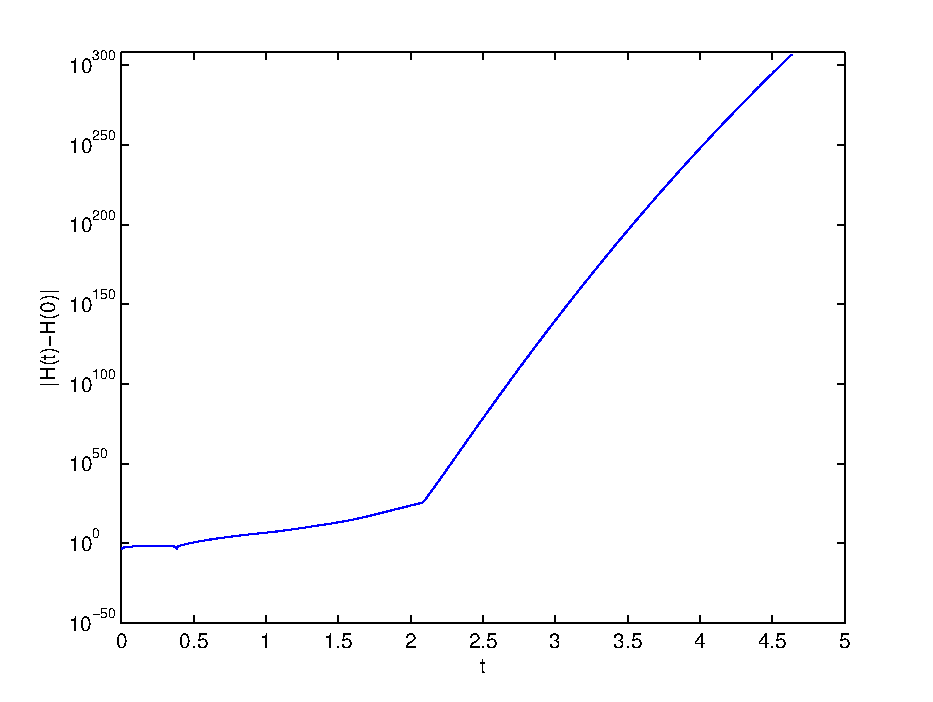
\includegraphics[width=0.45\textwidth]{03/Fig9-1.pdf}
  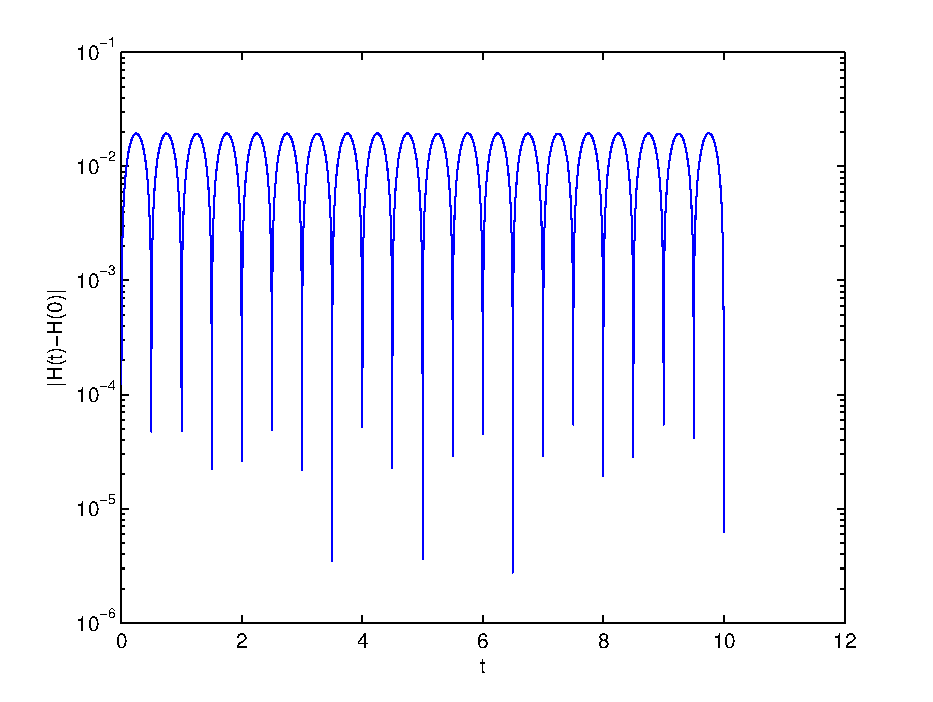
\includegraphics[width=0.45\textwidth]{03/Fig9-2.pdf}
  \caption{非线性波动方程 \eqref{eq:nonlinwave} 辛欧拉波形松弛方法无窗口加速(左图)和有窗口加速(右图)的比较}
  \label{fig:ex3seucom}
\end{figure}
\end{frame}

\begin{frame}{4.4 数值实验}
其次,考虑辛 Runge-Kutta 波形松弛方法. 取 $t_{\text{end}} = 10$, $N=20$, 步长为 $h = 1/100$, 波形松弛迭代次数为 $k=30$. 对于窗口加速方法,取每个时间窗口为 $0.1$. 图 \ref{fig:ex3srkcom} 展示了辛 Runge-Kutta 波形松弛方法无窗口加速(左图)和有窗口加速(右图)的比较.全局最大误差为 $3.7003e-05$.

\begin{figure}[h!]
  \centering
  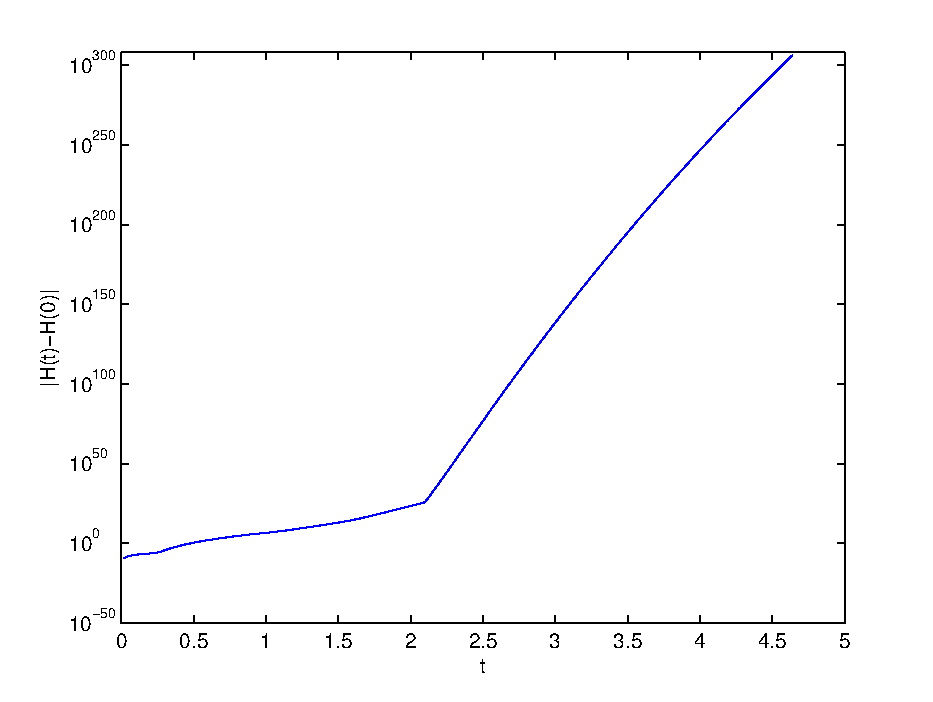
\includegraphics[width=0.45\textwidth]{03/Fig10-1.pdf}
  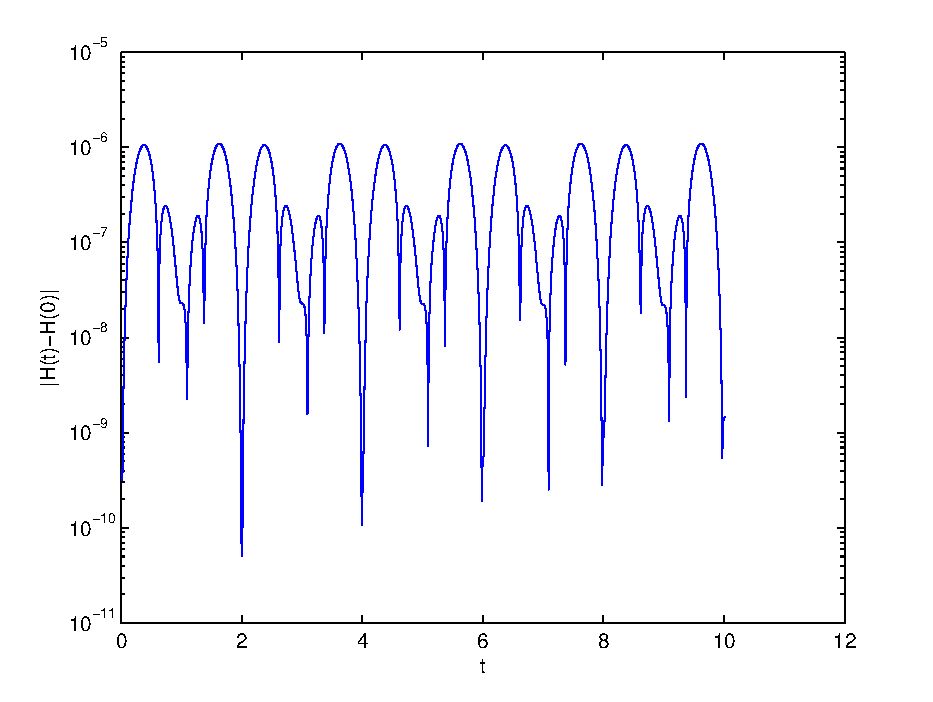
\includegraphics[width=0.45\textwidth]{03/Fig10-2.pdf}
  \caption{非线性波动方程 \eqref{eq:nonlinwave} 辛 Runge-Kutta 波形松弛方法无窗口加速(左图)和有窗口加速(右图)的比较}
  \label{fig:ex3srkcom}
\end{figure}
\end{frame}

\begin{frame}{4.4 数值实验}
其数值解的示意图如图 \ref{fig:wavefig}.

\begin{figure}[h!]
  \centering
  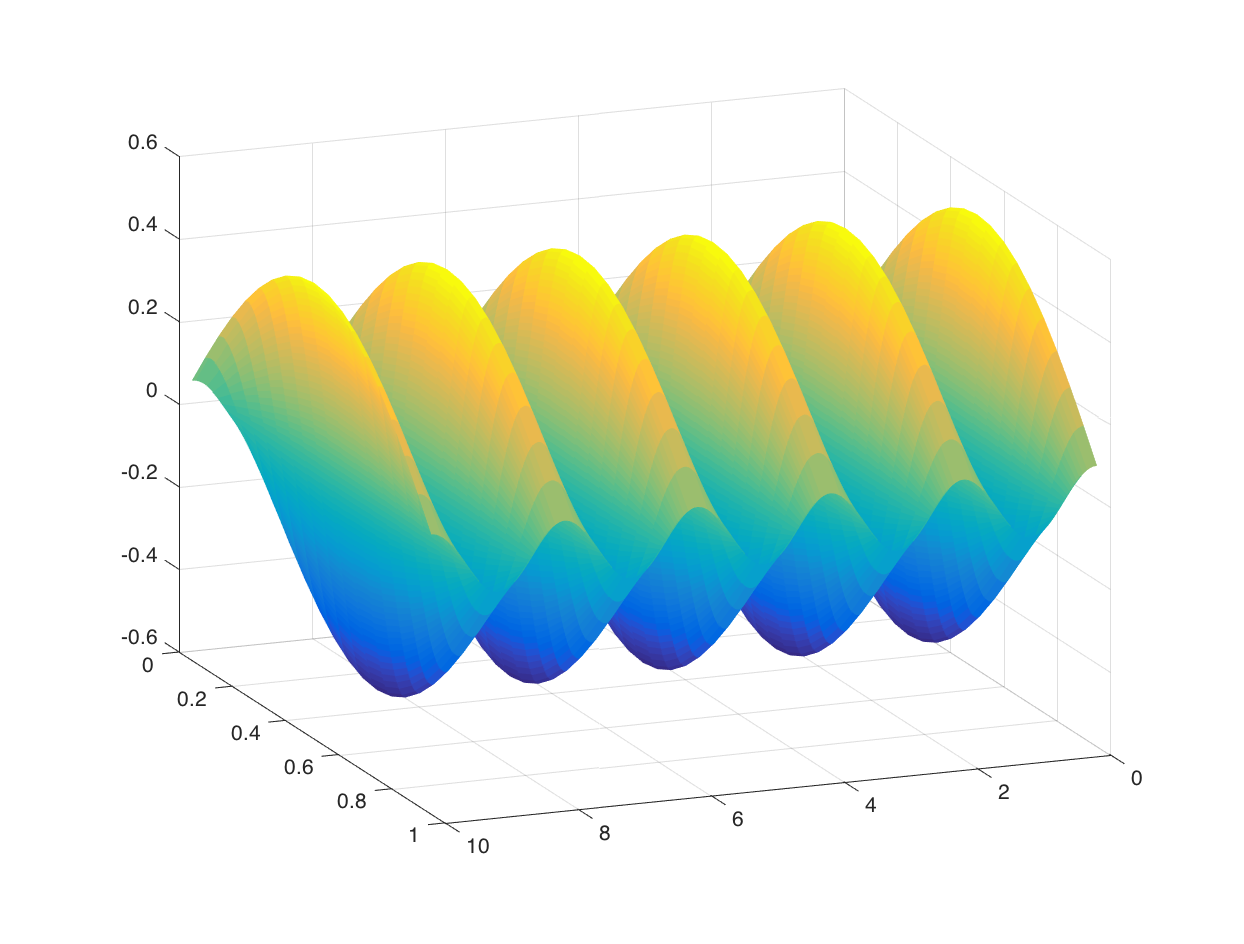
\includegraphics[width=0.7\textwidth]{03/wave.pdf}
  \caption{非线性波动方程的解示意图}
  \label{fig:wavefig}
\end{figure}
\end{frame}

\section{结论与展望}
\begin{frame}{5.1 结论}
\qquad 本博士论文主要围绕辛方法和李群方法进行了一些数值方法和解析方法的研究.具体内容包括以下几个方面:

(一) 在第~2~章,提出了一种新的求解带有齐次边界条件的电报方程的方法.该方法有效地结合了辛方法的特性,得到了
较好的数值结果.

(二) 在第~3~章,将复合变分准则应用到了 (2+1) 维拓展 QZK 方程.应用这些李点对称,得到了 (2+1) 维拓展 QZK 方程的一些性质.

(三) 在第~4~章,将波形松弛方法和辛方法应用到哈密尔顿系统上,提出了辛波形松弛方法,给波形松弛方法分裂函数的选取提供了一个可行性建议.并基于辛波形松弛方法,对隐式的 RK-MK 方法提出了一种改进方法.
\end{frame}

\begin{frame}{5.2 展望}
\qquad 在本博士论文的基础上,可以从如下几个方面进行进一步深入研究.

(一) 基于 RK-MK 方法,建立在流形上的保结构数值格式,这将给隐式 RK-MK 方法的使用提供理论依据.

(二) 对波形松弛方法进行修正和改进,使算法实用性更广泛.

(三) 对辛波形松弛方法设计并行算法,使波形松弛方法在工程应用中发挥作用.
\end{frame}

\section{审稿意见中的问题与回答}
\begin{frame}{审稿意见中的问题与回答}
\begin{block}{聂玉峰教授提出的问题}
解耦是执行并行算法期望的技巧,长时稳定是辛算法的优势;将二者结合起来进行算法设计,当进行并行设计时会面临什么样的困难?
\end{block}
答: 这是一个十分具有挑战性的开放问题,以本文的算法为例,算法 (P63,图 4-5) 采用了窗口技术,如果使用并行,使用 MPI 的框架,需要考虑如何分配资源,如何调度每个处理器,如何划分时间区域大小以达到较快的计算.

\qquad 此外,也可以从另外一个方面考虑,不斤斤计较精度,可能有更大的解耦,更好的并行度,这时的问题是如何保证收敛。
\end{frame}

\begin{frame}{审稿意见中的问题与回答}
\begin{block}{焦永昌教授提出的问题}
1. 为保持数学符号一致,建议将第9页(2-2)式下四行中的 ``n'' 修改为 ``d''.
\end{block}
答: 为了符号统一,对类似的问题作出了统一修改.

\begin{block}{焦永昌教授提出的问题}
2. 第17页第1行中的 ``$u=e^{-\frac{1}{2}kt}w$'' 应修改为 ``$u=e^{\frac{1}{2}kt}w$''; 第18页第11行和第20页第10行中的``时间格点''似乎应修改为``空间格点'';第23页第18行``较小的''后应增加 ``$\Delta t$''; 第36页倒数第3行中的 ``$\frac{\partial}{\partial x_i}$'' 应修改为 ``$\frac{\partial}{\partial x_1}$''.
\end{block}
答: 以上问题均在相应处作出了修改.
\end{frame}

\begin{frame}{审稿意见中的问题与回答}
\begin{block}{焦永昌教授提出的问题}
3. 第41页倒数第9行公式中求 $\Sigma$ 和运算后面的项与 $S$ 无关似乎有问题,请作者确认.
\end{block}
答:此处公式是正确的,但是叙述不完整,已经在论文中做了补充.
\end{frame}

%\begin{frame}{測試block環境}{副標題}
%    \begin{block}{BLOCK環境}
%        A quick brown fox jumps over the lazy dog.
%    \end{block} \pause
%
%    \begin{exampleblock}{EXAMPLEBLOCK環境}
%        A quick brown fox jumps over the lazy dog.
%    \end{exampleblock} \pause
%
%    \begin{alertblock}{ALERTBLOCK環境}
%        A quick brown fox jumps over the lazy dog.
%    \end{alertblock} 
%\end{frame}
%
%\begin{frame}{校訓}
%
%    \begin{block}{西安交通大學校訓}
%        \centering \Huge
%        精勤求學
%        \\ \pause
%        敦篤勵志
%        \\ \pause
%        果毅力行
%        \\ \pause
%        忠恕任事
%    \end{block}
%
%\end{frame}

\begin{frame}{致谢}
\qquad 人生路漫漫,不觉间来交大已经十个春秋.在这段短暂又漫长的人生路里,是这所百年名校教诲培养着我,指引我前进.

\qquad 我在这里首先要感谢我的导师蒋耀林教授,我成长的每一步和他是分不开的.是老师教导我如何正确选择人生道路,让我少走些弯路;
是老师纠正我性格中的每一个缺点,让我变得越来越坚强;是老师教给我``追求=坚持''的等式,让我驶向前方的道路是意志坚定;
是老师给了我一个相对自由的学习空间,让我这些年不受世俗所累安心学习.
蒋老师付出的每一分汗水,每一次教诲我都铭记在心,并以此作为指引我走好前方的路.

\qquad 感谢学位论文评审专家和答辩委员会的专家教授!

\qquad 还要感谢同师门的师兄弟姐妹们,是他们陪我走过数个春秋,翻越一座座高山.路漫漫其修远兮,吾将上下而求索.我会在今后的人生道路上,带着积累多年的知识与本领,继续辉煌地走好每一步.
\end{frame}

\end{document}


